\chapter{Математическая модель БОЭП как объекта управления} \label{ch:ch3}

Оптико-электронный прибор (ОЭП) вертолетного базирования имеет тепловизионный и телевизионный каналы, лазерный дальномер. Кроме того, на борту устанавливают оптико-электронную систему постановки помех (СОЭП).  Управление направлением линии визирования осуществляется перемещением всего оптико-электронного блока. Для ОЭП и СОЭП конструктивно оптико-электронный блок представляет собой блок, в котором размещены оптические приборы, вращающийся по углу места внутри вилки, вращающейся по углу азимута 
(рисунок~\ref{fig:device}, кинематическая схема на рисунке~\ref{fig:kinematic}). 
На осях вращения размещены моментные двигатели и датчики углов. ОЭП установлен в носовой части вертолета, СОЭП устанавливается в хвостовой части и на балках 
(рисунок~\ref{fig:helicopter}).

При проектировании ОЭП и СОЭП возникли задачи построения адекватной математической модели, синтеза системы управления направлением линии визирования и построения компьютерной имитационной модели ОЭП и СОЭП. Решение этих задач является продолжением работ [3/15-18]. Математическая модель строится на основе применения уравнений Лагранжа II-го рода с использованием смешанного метода Жильбера. Разработаны алгоритмы управления, обеспечивающие требуемые точностные и динамические характеристики СОЭП для режима слежения и наведения. Исследование динамических свойств СОЭП проводится с использованием компьютерной имитационной модели. Использование метода математического моделирования при проектировании бортовых СОЭП позволяет обеспечить достижение заложенных технических требований по параметрам системы, сократить сроки разработки, настройки и испытаний изделия. Компьютерная имитационная модель верифицирована по результатам настройки опытного образца.

\begin{landscape}
\section{Принципиальная схема} \label{ch:ch3/sect1}

\begin{figure}[ht]
	\centering
	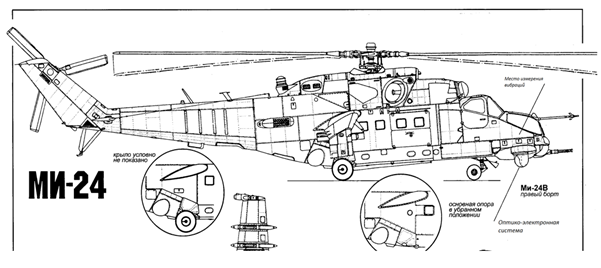
\includegraphics[width=0.9\linewidth]{img-15} 
	\caption{Принципиальная схема расположения на борту}
	\label{fig:helicopter}
\end{figure}

\begin{figure}[ht]
	\centering
	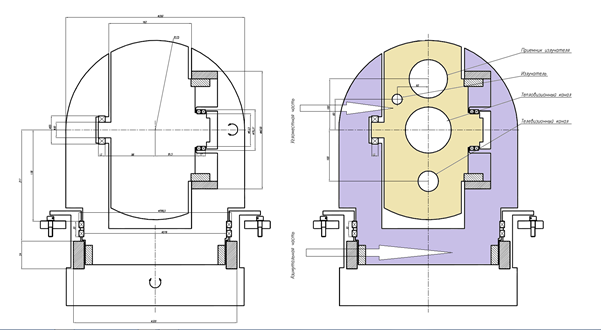
\includegraphics[width=0.9\linewidth]{img-16} 
	\caption{Общий вид изделия}
	\label{fig:device}
\end{figure}
\end{landscape}

\section{Механическая модель} \label{ch:ch3/sect2}

Исходя из анализа конструкции ОЭП для управления линией визирования оптико-электронного блока – объекта управления (ОУ) и движения вертолета (ЛА), на котором он установлен, приняты основные допущения, выбраны системы координат и определены исходные данные, необходимые для построения математической модели. ОУ.

\begin{figure}[ht]
	\centering
	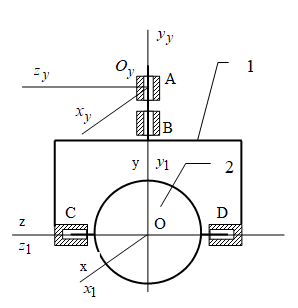
\includegraphics[]{img-17} 
	\caption{Кинематическая схема}
	\label{fig:kinematic}
\end{figure}

\subsection{Основные допущения, системы координат} \label{sec:ch3/sec3}

\begin{enumerate}
	\item ОУ моделируется двумя абсолютно твердыми телами:
	\begin{itemize}
		\item 1–е тело объединяет все элементы, вращающиеся по углу азимута вокруг оси АВ (рисунок \ref{fig:kinematic}) в неограниченном диапазоне (более $360_0$). Тело 1 (вилка) совершает вращательное движение вокруг оси АВ под действием вращающего момента, создаваемого моментным двигателем.
		\item 2–е тело (оптико-электронный блок) объединяет все элементы, вращающиеся по углу места вокруг оси CD (рисунок \ref{fig:device}). Тело 2 (оптико-электронный блок) вращается относительно тела 1 вокруг оси CD под действием вращающего момента, создаваемого другим моментным двигателем.
	\end{itemize}
	\item Ось вращения 2-го тела перпендикулярна оси вращения 1-го тела и пересекается с ней: $AB\perp CD$, т.$O \in AB$, т.$O \in CD$
	\item Инерциальная система координат, система координат связанная с вертолетом (ЛА) и установочная система координат выбраны в соответствии с принципиальной схемой расположения на борту (рисунок \ref{fig:helicopter}). Их положение и кинематические характеристики  определены выражениями (3.1)-(3.14).
	\item Система координат $O_{x_1y_1z_1}$ (рисунок \ref{fig:coord/3.4}) жестко связана с 1-м телом. 
	\begin{figure}[ht]
		\centering
		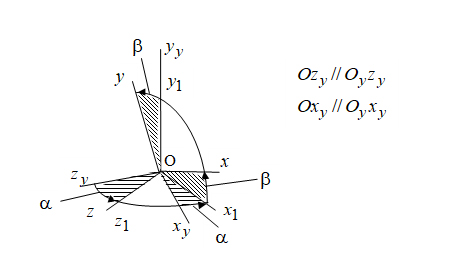
\includegraphics[]{img-18} 
		\caption{Кинематическая схема}
		\label{fig:coord/3.4}
	\end{figure}

	Ось $O_{y_1}$ направлена по оси вращения АВ, ось $O_{z_1}$ направлена по оси вращения CD, ось $O_{x_1}$ дополняет указанные оси до правой системы координат. Точка O находится на пересечении осей АВ и CD. Положение точки О в установочной системе координат определяется радиусом-вектором
	\begin{equation}
	\label{eq:p3:1}
	\begin{alignedat}{2}
	\bar{r}_0 = \bar{e}_y\tilde{r}_0 ,
	\end{alignedat}
	\end{equation}
	где $\tilde{r}_0 = (0 -l 0)^T$.
	
	Орты осей $O_{x_1y_1z_1}$ обозначим $\bar{i}_1$, $\bar{j}_1$, $\bar{k}_1$ и составим из них базисную строку $\bar{e}_1 = (\bar{i}_1 \bar{j}_1 \bar{k}_1)$. Связь между базисными строками $\bar{e}_y$ и $\bar{e}_1$ определяются матрицей $A_1$:
	\begin{equation}
	\label{eq:p3:2}
	\begin{alignedat}{2}
	\bar{e}_y = \bar{e}_1	A_1 ,
	\end{alignedat}
	\end{equation}
	где  \( A_{1}= \left( \begin{matrix}
	cos \alpha   &  0  &  -sin \alpha \\
	0  &  1  &  0\\
	sin \alpha   &  0  &  cos \alpha \\
	\end{matrix}
	\right)  \) .\par
	
	Масса 1-го тела равна  \( m_{1} \) , положение центра масс в системе координат  \( Ox_{1}y_{1}z_{1} \)  определяется радиусом-вектором\par
	
	\begin{equation}
	\label{eq:p3:3}
	\begin{alignedat}{2}
	r_{с_{1}}=e_{1}r_{с_{1}},
	\end{alignedat}
	\end{equation}
	
	где  \( r_{с_{1}}= \left( \begin{matrix}
	x_{с_{1}}  &  y_{с_{1}}  &  z_{с_{1}}\\
	\end{matrix}
	\right) ^{T} \) .\par
	Введем следующие обозначения для осевых и центробежных моментов инерции 1-го тела:\par
	
	\( J_{x_{1}}=A_{1},J_{y_{1}}=B_{1},J_{z_{1}}=C_{1},J_{x_{1}y_{1}}=F_{1},J_{x_{1}z_{1}}=E_{1},J_{y_{1}z_{1}}=D_{1} \) ,\par
	
	тогда его тензор инерции\par
	
	\begin{equation}
	\label{eq:p3:4}
	\begin{alignedat}{2}
	J_{1}= \left( \begin{matrix}
	A_{1}  &  -F_{1}  &  -E_{1}\\
	-F_{1}  &  B_{1}  &  -D_{1}\\
	-E_{1}  &  -D_{1}  &  C_{1}\\
	\end{matrix}
	\right) 
	\end{alignedat}
	\end{equation}
		
	\item Оси  \( Oxyz \)  (рисунок \ref{fig:coord/3.4}) жестко связаны с телом 2: ось  \( Ox \)  направлена по оптической оси, ось  \( Oz \)  совпадает с осью вращения \textit{CD}, ось  \( Oy \)  дополняет указанные оси до правой системы координат.\par
	
	Орты осей  \( Ox_{1}y_{1}z_{1} \)  обозначим  \( i,j,k_{1} \)  и составим из них базисную строку  \( е= \left( \begin{matrix}
	i  &  j  &  k\\
	\end{matrix}
	\right)  \) . Связь между базисными строками  \( e \)  и  \( e_{1} \)  определяется матрицей  \( A_{2} \) :\par
	
	\begin{equation}
	\label{eq:p3:5}
	\begin{alignedat}{2}
	e_{1}=eA_{2},
	\end{alignedat}
	\end{equation}
	
	где  \( A_{2}= \left( \begin{matrix}
	cos \beta   &  sin \beta   &  0\\
	-sin \beta   &  cos \beta   &  0\\
	0  &  0  &  1\\
	\end{matrix}
	\right)  \) .\par
	
	Масса 2-го тела равна  \( m_{2} \) , положение центра масс в системе координат  \( Oxyz \)  определяется радиусом-вектором\par
	
	\begin{equation}
	\label{eq:p3:6}
	\begin{alignedat}{2}
	r_{с_{2}}=e r_{с_{2}},
	\end{alignedat}
	\end{equation}
	
	где  \( r_{с_{2}}= \left( \begin{matrix}
	x_{с_{2}}  &  y_{с_{2}}  &  z_{с_{2}}\\
	\end{matrix}
	\right) ^{T} \) .\par
	
	Введем следующие обозначения для осевых и центробежных моментов инерции 2-го тела:\par
	
	\( J_{x_{}}=A_{2},J_{y}=B_{2},J_{z}=C_{2},J_{x_{2}y_{2}}=F_{2},J_{x_{2}z_{2}}=E_{2},J_{y_{2}z_{2}}=D_{2} \) ,\par
	
	тогда его тензор инерции\par
	
	\begin{equation}
	\label{eq:p3:7}
	\begin{alignedat}{2}
	J_{2}= \left( \begin{matrix}
	A_{2}  &  -F_{2}  &  -E_{2}\\
	-F_{2}  &  B_{2}  &  -D_{2}\\
	-E_{2}  &  -D_{2}  &  C_{2}\\
	\end{matrix}
	\right) 
	\end{alignedat}
	\end{equation}	
	\item Движение ЛА происходит в однородном поле силы тяжести.
\end{enumerate}


\subsection{Геометрия масс} \label{sec:ch3/sec4}

По рабочим чертежам в среде Solid Works получены массовые характеристики ОУ. Их обозначения и величины приведены в таблице ниже (таблица \ref{tab:MASS/3.1}).



{
	\setlength\extrarowheight{3pt}
	\begin{longtable}{p{0.66in}p{1.94in}p{0.71in}p{0.29in}p{0.49in}p{0.39in}p{0.66in}}
		\caption{Массовые характеристики ОУ}%
		\label{tab:MASS/3.1}% label всегда желательно идти после caption
		\\
\hline
		%row no:1
		\multicolumn{1}{|p{0.66in}}{№ п/п} & 
		\multicolumn{1}{|p{1.94in}}{Наименование} & 
		\multicolumn{1}{|p{0.71in}}{Обозначение} & 
		\multicolumn{3}{|p{1.57in}}{Величина} & 
		\multicolumn{1}{|p{0.66in}|}{Размерность} \\
		\hline
		%row no:2
		\multicolumn{1}{|p{0.66in}}{1} & 
		\multicolumn{1}{|p{1.94in}}{2} & 
		\multicolumn{1}{|p{0.71in}}{3} & 
		\multicolumn{3}{|p{1.57in}}{4} & 
		\multicolumn{1}{|p{0.66in}|}{5} \\
		\hline
		%row no:3
		\multicolumn{1}{|p{0.66in}}{1} & 
		\multicolumn{1}{|p{1.94in}}{Координаты центра прибора относительно центра масс носителя \par } & 
		\multicolumn{1}{|p{0.71in}}{Y\textsubscript{0} \par X\textsubscript{0} \par Z\textsubscript{0}} & 
		\multicolumn{1}{|p{0.29in}}{-0.5 \par -0.5 \par -2} & 
		\multicolumn{1}{|p{0.49in}}{0 \par -8.422 \par 0} & 
		\multicolumn{1}{|p{0.39in}}{-0.5 \par -0.5 \par 2} & 
		\multicolumn{1}{|p{0.66in}|}{\textit{м}} \\
		\hline
		%row no:4
		\multicolumn{1}{|p{0.66in}}{2} & 
		\multicolumn{1}{|p{1.94in}}{\multirowcell{2}{}{\begin{tabular}{p{1.94in}}Масса 1-го тела вращения (по азимуту), координаты его центра масс, осевые и центробежные моменты инерции\\(Ось вращения – Y)\\\end{tabular}}} & 
		\multicolumn{1}{|p{0.71in}}{m\textsubscript{1}} & 
		\multicolumn{3}{|p{1.57in}}{15.7} & 
		\multicolumn{1}{|p{0.66in}|}{\textit{кг}} \\
		\hline
		%row no:5
		\multicolumn{1}{|p{0.66in}}{3} & 
		\multicolumn{1}{|p{1.94in}}{} & 
		\multicolumn{1}{|p{0.71in}}{x\textsubscript{C1}} & 
		\multicolumn{3}{|p{1.57in}}{-2.82} & 
		\multicolumn{1}{|p{0.66in}|}{\textit{мм}} \\
		\hline
		%row no:6
		\multicolumn{1}{|p{0.66in}}{4} & 
		\multicolumn{1}{|p{1.94in}}{} & 
		\multicolumn{1}{|p{0.71in}}{z\textsubscript{C1}} & 
		\multicolumn{3}{|p{1.57in}}{8.64} & 
		\multicolumn{1}{|p{0.66in}|}{\textit{мм}} \\
		\hline
		%row no:7
		\multicolumn{1}{|p{0.66in}}{5} & 
		\multicolumn{1}{|p{1.94in}}{} & 
		\multicolumn{1}{|p{0.71in}}{y\textsubscript{C1}} & 
		\multicolumn{3}{|p{1.57in}}{-95.03} & 
		\multicolumn{1}{|p{0.66in}|}{\textit{мм}} \\
		\hline
		%row no:8
		\multicolumn{1}{|p{0.66in}}{6} & 
		\multicolumn{1}{|p{1.94in}}{} & 
		\multicolumn{1}{|p{0.71in}}{ \( J_{x_{1}}=A_{1} \) } & 
		\multicolumn{3}{|p{1.57in}}{212} & 
		\multicolumn{1}{|p{0.66in}|}{\textit{гр м\textsuperscript{2}}} \\
		\hline
		%row no:9
		\multicolumn{1}{|p{0.66in}}{7} & 
		\multicolumn{1}{|p{1.94in}}{} & 
		\multicolumn{1}{|p{0.71in}}{ \( J_{y_{1}}=B_{1} \) } & 
		\multicolumn{3}{|p{1.57in}}{311.8} & 
		\multicolumn{1}{|p{0.66in}|}{\textit{гр м\textsuperscript{2}}} \\
		\hline
		%row no:10
		\multicolumn{1}{|p{0.66in}}{12} & 
		\multicolumn{1}{|p{1.94in}}{\multirowcell{2}{}{\begin{tabular}{p{1.94in}}Масса 2-го тела вращения (по углу места), координаты его центра масс, осевые и центробежные моменты инерции\\(Ось вращения - Z)\\\end{tabular}}} & 
		\multicolumn{1}{|p{0.71in}}{ \( m_{2} \) } & 
		\multicolumn{3}{|p{1.57in}}{1130.85} & 
		\multicolumn{1}{|p{0.66in}|}{\textit{гр}} \\
		\hline
		%row no:11
		\multicolumn{1}{|p{0.66in}}{13} & 
		\multicolumn{1}{|p{1.94in}}{} & 
		\multicolumn{1}{|p{0.71in}}{ \( x_{C_{2}} \) } & 
		\multicolumn{3}{|p{1.57in}}{0} & 
		\multicolumn{1}{|p{0.66in}|}{\textit{мм}} \\
		\hline
		%row no:12
		\multicolumn{1}{|p{0.66in}}{14} & 
		\multicolumn{1}{|p{1.94in}}{} & 
		\multicolumn{1}{|p{0.71in}}{ \( y_{C_{2}} \) } & 
		\multicolumn{3}{|p{1.57in}}{14.8} & 
		\multicolumn{1}{|p{0.66in}|}{\textit{мм}} \\
		\hline
		%row no:13
		\multicolumn{1}{|p{0.66in}}{15} & 
		\multicolumn{1}{|p{1.94in}}{} & 
		\multicolumn{1}{|p{0.71in}}{ \( z_{C_{2}} \) } & 
		\multicolumn{3}{|p{1.57in}}{-8} & 
		\multicolumn{1}{|p{0.66in}|}{\textit{мм}} \\
		\hline
		%row no:14
		\multicolumn{1}{|p{0.66in}}{16} & 
		\multicolumn{1}{|p{1.94in}}{} & 
		\multicolumn{1}{|p{0.71in}}{ \( J_{x_{2}}=A_{2} \) } & 
		\multicolumn{3}{|p{1.57in}}{3.3} & 
		\multicolumn{1}{|p{0.66in}|}{\textit{гр м\textsuperscript{2}}} \\
		\hline
		%row no:15
		\multicolumn{1}{|p{0.66in}}{17} & 
		\multicolumn{1}{|p{1.94in}}{} & 
		\multicolumn{1}{|p{0.71in}}{ \( J_{y_{2}}=B_{2} \) } & 
		\multicolumn{3}{|p{1.57in}}{7.5} & 
		\multicolumn{1}{|p{0.66in}|}{\textit{гр м\textsuperscript{2}}} \\
		\hline
		%row no:16
		\multicolumn{1}{|p{0.66in}}{18} & 
		\multicolumn{1}{|p{1.94in}}{} & 
		\multicolumn{1}{|p{0.71in}}{ \( J_{z_{2}}=C_{2} \) } & 
		\multicolumn{3}{|p{1.57in}}{8.4} & 
		\multicolumn{1}{|p{0.66in}|}{\textit{гр м\textsuperscript{2}}} \\
		\hline
		
\end{longtable}}

%%%%%%%%%%%%%%%%%%%% Table No: 4 ends here %%%%%%%%%%%%%%%%%%%%

\section{Составление уравнений динамической модели ОУ} \label{ch:ch3/sect5}


\subsection{Вычисление кинетической энергии} \label{sec:ch3/sec6}

\subsection{Вычисление обобщенных сил} \label{sec:ch3/sec7}

\subsection{Составление уравнений динамической модели ОУ} \label{sec:ch3/sec8}


\section{Модель привода} \label{ch:ch3/sect9}

\section{Линеаризованная система} \label{ch:ch3/sect10}

\section{Выводы по главе} \label{ch:ch3/sect11}


Некоторый текст.

\clearpage